\documentclass[11pt, addpoints, answers]{exam}

\usepackage{amsmath, amssymb, amsthm}
\usepackage{xcolor}
\usepackage{graphicx}
\usepackage{graphics}
\usepackage{enumerate}


\usepackage{tikz}
\usepackage{tikz-qtree}
\usetikzlibrary{graphs}
\usetikzlibrary{arrows.meta}
\usepackage{listings}   
\usepackage{caption}
\makeatletter
\makeatother


\usepackage{algorithm}
\usepackage{algorithmic}




% For inserting code snippets.
\usepackage{listings}
\lstset{
	columns = fixed,
	basewidth = {0.5em},
	breaklines = true,
	backgroundcolor = \color{white},
	keywordstyle = \color[RGB]{40, 40, 255},
	numberstyle = \footnotesize\color{darkgray},
	commentstyle = \ttfamily\color{violet},
	basicstyle = \ttfamily,
	stringstyle = \ttfamily\color[RGB]{128, 0, 0},
	showstringspaces = false,
	language = {[11]C++},
	escapechar = \@
}
\lstnewenvironment{cpp}[1][]{\lstset{language = {[11]C++}, #1}}{}

\usepackage{tikz}
\usetikzlibrary{positioning}
% headers, footers, titles
\newcommand{\CourseName}{CS101 Algorithms and Data Structures}
\newcommand{\HomeworkNO}{Homework 8}
\newcommand{\DueDate}{Due date: 23:59, December 10th, 2023}

\pagestyle{headandfoot}
\runningheadrule
\runningheader{\CourseName}{\HomeworkNO}{\DueDate}
\runningfooter{}{\thepage}{}

\title{
	\CourseName\\
	Fall 2023\\
	\HomeworkNO\\
}
\author{}
\date{\DueDate}

% formats of questions, choices, points, etc.
\qformat{\bf\thequestion. (\totalpoints\ points) \thequestiontitle\hfill}
\pointname{'}
\CorrectChoiceEmphasis{\bf\color{blue}}
\SolutionEmphasis{\color{blue}}

% We frequently use this font.
\newcommand{\ttt}{\texttt}

\begin{document}

\maketitle

\begin{enumerate}
	\item Please write your solutions in English.
	\item Submit your solutions to gradescope.com.
	\item Set your FULL name to your Chinese name and your STUDENT ID correctly in Account Settings.
	\item If you want to submit a handwritten version, scan it clearly. \ttt{CamScanner} is recommended.
	\item When submitting, match your solutions to the problems correctly.
	\item No late submission will be accepted.
	\item Violations to any of the above may result in zero points.
\end{enumerate}

\begin{questions}

	\titledquestion{Multiple Choices}

Each question has \textbf{one or more} correct answer(s). Select all the correct answer(s). For each question, you will get 0 points if you select one or more wrong answers, but you will get 1 point if you select a non-empty subset of the correct answers.

Write your answers in the following table.

%%%%%%%%%%%%%%%%%%%%%%%%%%%%%%%%%%%%%%%%%%%%%%%%%%%%%%%%%%%%%%%%%%%%%%%%%%%
% Note: The `LaTeX' way to answer a multiple-choices question is to replace `\choice'
% with `\CorrectChoice', as what you did in the first question. However, there are still
% many students who would like to handwrite their homework. To make TA's work easier,
% you have to fill your selected choices in the table below, no matter whether you use 
% LaTeX or not.
%%%%%%%%%%%%%%%%%%%%%%%%%%%%%%%%%%%%%%%%%%%%%%%%%%%%%%%%%%%%%%%%%%%%%%%%%%%

\begin{table}[htbp]
    \centering
    \begin{tabular}{|p{2cm}|p{2cm}|p{2cm}|p{2cm}|}
        \hline
        (a) & (b) & (c) & (d) \\
        \hline
        %%%%%%%%%%%%%%%%%%%%%%%%%%%%%%%%%%%%%%%%%%%%%%%%%%%%%%%%%%
        % YOUR ANSWER HERE.
        AD  & BCD & AB  & D   \\
        %%%%%%%%%%%%%%%%%%%%%%%%%%%%%%%%%%%%%%%%%%%%%%%%%%%%%%%%%%
        \hline
    \end{tabular}
\end{table}

\begin{parts}
    \part[2] Which of the following operations on a \textbf{Linked List} take constant time?

    \begin{choices}
        \CorrectChoice Given a pointer $h$ which points to the head node of a linked list, we want to erase the head node.
        \choice Given a pointer $h$ which points to the head node of a linked list, we want to gain access to the last element of the linked list.
        \choice Given a pointer $p$ which points to a node in a linked list, we want to gain access the previous node of $p$.
        \CorrectChoice Given a pointer $p$ which points to a node in a linked list, we want to insert an element after $p$.
    \end{choices}

    \part[2] Which of the following statements about arrays and linked-lists are true?

    \begin{choices}
        \choice Inserting an element into the middle of an array takes constant time.
        \CorrectChoice A doubly linked list consumes more memory than a (singly) linked list of the same length.
        \CorrectChoice Given a pointer to some node in a doubly linked list, we are able to gain access to every node of it.
        \CorrectChoice Given a pointer to any node in a linked list, we are able to gain access to the last node.
    \end{choices}

    \part[2] Please evaluate the following reverse-Polish expressions. Which of them are legal reverse-Polish expressions and gives a result greater than 0?

    \begin{choices}
        \CorrectChoice \ttt{2 3 2 * + 1 /}
        \CorrectChoice \ttt{1 2 4 - - 3 *}
        \choice \ttt{1 * 2 - 1 + 5}
        \choice \ttt{2 4 3 1 + * -}
    \end{choices}

    \part[2] Assume we implement a queue with a circular array indexed from $0$ to $n-1$. Now the \ttt{front} pointer is at index $a$, and the \ttt{back} pointer is at index $b$. Which of the following best describes the number of the elements in the queue?

    \begin{choices}
        \choice $b-a+1$
        \choice $|b-a+1|$
        \choice $b-a+1+n$
        \CorrectChoice $(b-a+1+n) \mod n$
    \end{choices}


\end{parts}

	\newpage
	\titledquestion{Graph traversal}
Consider the following undirected graph.
\begin{center}
	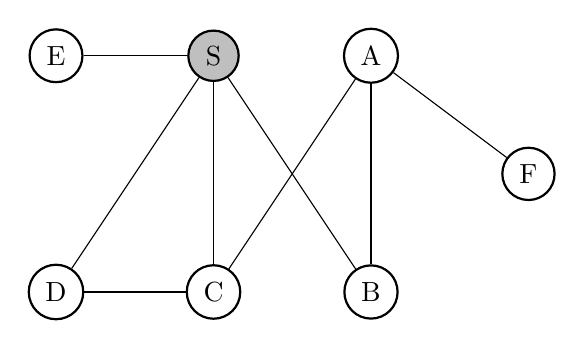
\begin{tikzpicture}
		\begin{scope}[every node/.style = {circle, thick, draw}]
			\node[fill={rgb:black,1;white,3}] (S) at (0,0) {S};
			\node (A) at (2,0) {A};
			\node (B) at (2, -3) {B};
			\node (C) at (0, -3) {C};
			\node (D) at (-2, -3) {D};
			\node (E) at (-2, 0) {E};
			\node (F) at (4, -1.5) {F};
		\end{scope}
		\begin{scope}[>={Stealth[black]}]
			\path[-] (S) edge (E);
			\path[-] (S) edge (D);
			\path[-] (S) edge (C);
			\path[-] (S) edge (B);
			\path[-] (C) edge (D);
			\path[-] (B) edge (A);
			\path[-] (A) edge (C);
			\path[-] (A) edge (F);

		\end{scope}
	\end{tikzpicture}

\end{center}

\begin{parts}
	\part[3] Give the adjacency list for the graph. You should write the node in alphabetical order. (Leave it blank if the node has no neighbour).\\
	\[
		\begin{array}{ll}
			adj(S) & = [\fillin[E, D, C, B]], \\
			adj(A) & = [\fillin[F, C, B]],    \\
			adj(B) & = [\fillin[A, S]],       \\
			adj(C) & = [\fillin[A, D, S]],    \\
			adj(D) & = [\fillin[C, S]],       \\
			adj(E) & = [\fillin[S]],          \\
			adj(F) & = [\fillin[A]],          \\
		\end{array}
	\]
	\part[3] Give the visited node order using the above adjacency list for Breadth First Search  starting with \(S\).(Each nodes only visit once)
	\begin{solution}
		\[ S \rightarrow E \rightarrow D \rightarrow C \rightarrow B \rightarrow A \rightarrow F \]
	\end{solution}
	\part[3] Give the visited node order using the above adjacency list for Depth First Search starting with \(S\). (Each nodes only visit once)\\
	Notes: The adjacency list should be inserted into the stack in reverse order. For example, if you access a point with the adjacency list [A, S], then after pushing the adjacency list onto the stack, A will be on the top of the stack
	\begin{solution}
		\[ S \rightarrow B \rightarrow A \rightarrow F \rightarrow C \rightarrow D \rightarrow E \]
	\end{solution}
\end{parts}

	\newpage
	\titledquestion{Disjoint Set practice}

Let's performing a series of merge opertions on a disjoint set structure.
Please show the final disjoint set tree for each of the following optimization strategies.

\newcommand{\SET}[1]{\{#1\}}

\begin{enumerate}[{\bf op} 1.]
        \item initialize: $\SET{1}, \SET{2}, \SET{3}, \SET{4}, \SET{5}, \SET{6}, \SET{7}, \SET{8}, \SET{9}$
        \item merge 1,4
        \item merge 3,2
        \item merge 7,6
        \item merge 7,3
        \item find 2
        \item merge 5,8
        \item merge 1,9
        \item merge 9,8
        \item merge 9,2
        \item find 6
\end{enumerate}

\begin{parts}
        \part[2] Only with union-by-height optimization. (When two trees have the same height, the set specified first in the union will be the root of the merged set.)

        \begin{solution}
                \begin{center}
                        \begin{tikzpicture}[level distance=1.5cm,
                                        level 1/.style={sibling distance=3cm},
                                        level 2/.style={sibling distance=1.5cm}]
                                \node {1}
                                child {node {5}
                                                child {node {8}}}
                                child {node {7}
                                                child {node {3}
                                                                child {node {2}}}
                                                child {node {6}}}
                                child {node {9}}
                                child {node {4}};
                        \end{tikzpicture}
                \end{center}
        \end{solution}


        \part[2] Only with path compression (The set specified first in the union will always be the root of the merged set).

        \begin{solution}
                \begin{center}
                        \begin{tikzpicture}[level distance=1.5cm,
                                        level 1/.style={sibling distance=3cm},
                                        level 2/.style={sibling distance=1.5cm}]
                                \node {1}
                                child {node {5}
                                                child {node {8}}}
                                child {node {7}
                                                child {node {3}}
                                                child {node {2}}}
                                child {node {9}}
                                child {node {4}}
                                child {node {6}};
                        \end{tikzpicture}
                \end{center}
        \end{solution}
\end{parts}


    \newpage
    \titledquestion{In Or Not In?}[6]

In this problem, we want you to run Kruskal's algorithm on the given graph. For each edge, indicate either the order it was added to the Minimum Spanning Tree (MST) or if it's not in the MST. For instance, if edge $(u,v)$ was the $3$rd edge added to the MST, mark ``In MST'' and write $3$ in the corresponding order box. If an edge is not in the MST, mark ``Not In MST'' and leave the order box blank.


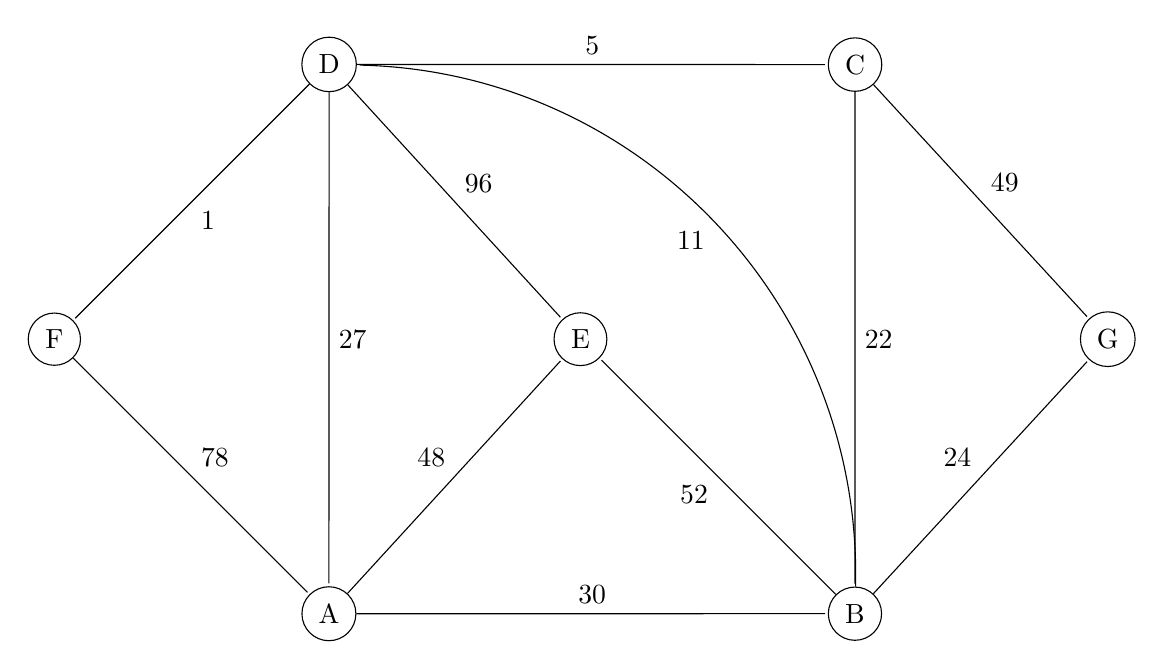
\begin{tikzpicture}[shorten >=1pt,node distance=2cm,auto] 
   \node[circle,draw] (F)   {F}; 
   \node[circle,draw] (D) [above right=3cm and 3cm of F] {D}; 
   \node[circle,draw] (A) [below right=3cm and 3cm of F] {A}; 
   \node[circle,draw] (E) [right=6cm of F] {E};
   \node[circle,draw] (C) [above right=3cm and 3cm of E] {C}; 
   \node[circle,draw] (B) [below right=3cm and 3cm of E] {B};
   \node[circle,draw] (G) [right=6cm of E] {G}; 
    \path[-] 
    (D) edge node {1} (F)
    (D) edge node {27} (A)
    (F) edge node {78} (A)
    (A) edge node {48} (E)
    (D) edge node {96} (E)
    (A) edge node {30} (B)
    (B) edge node {52} (E)
    (B) edge [bend right=45] node {11} (D)
    (D) edge node {5} (C)
    (C) edge node {22} (B)
    (C) edge node {49} (G)
    (B) edge node {24} (G);
\end{tikzpicture}

You should write your answer in the table below:

\begin{table}[htbp]
\Large
\begin{tabular}{|l|l|c|}
\hline
Edge & Whether In MST & Order \\ \hline
AB   & \begin{oneparcheckboxes}\choice Not In MST\space\choice In MST\end{oneparcheckboxes} &       \\ \hline
AD   & \begin{oneparcheckboxes}\choice Not In MST\space\choice In MST\end{oneparcheckboxes} &       \\ \hline
AE   & \begin{oneparcheckboxes}\choice Not In MST\space\choice In MST\end{oneparcheckboxes} &       \\ \hline
AF   & \begin{oneparcheckboxes}\choice Not In MST\space\choice In MST\end{oneparcheckboxes} &       \\ \hline
BC   & \begin{oneparcheckboxes}\choice Not In MST\space\choice In MST\end{oneparcheckboxes} &       \\ \hline
BD   & \begin{oneparcheckboxes}\choice Not In MST\space\choice In MST\end{oneparcheckboxes} &       \\ \hline
BE   & \begin{oneparcheckboxes}\choice Not In MST\space\choice In MST\end{oneparcheckboxes} &       \\ \hline
BG   & \begin{oneparcheckboxes}\choice Not In MST\space\choice In MST\end{oneparcheckboxes} &       \\ \hline
CD   & \begin{oneparcheckboxes}\choice Not In MST\space\choice In MST\end{oneparcheckboxes} &       \\ \hline
CG   & \begin{oneparcheckboxes}\choice Not In MST\space\choice In MST\end{oneparcheckboxes} &       \\ \hline
DE   & \begin{oneparcheckboxes}\choice Not In MST\space\choice In MST\end{oneparcheckboxes} &       \\ \hline
DF   & \begin{oneparcheckboxes}\choice Not In MST\space\choice In MST\end{oneparcheckboxes} &       \\ \hline
\end{tabular}
\end{table}
    \newpage
    \titledquestion{Traffic Network}[8]

In SC101 country, there are $n$ cities and $m$ \textbf{broken} roads, with each broken road connecting two different cities. You can consider this as a graph $G=(V, E)$. 

Now the government wants to build a traffic net in the SC101 country. There are $2$ crucial steps to take in constructing this traffic network:
\begin{enumerate}
    \item Establish an airport in the $i$-th city with a cost of $a_i$
    \item Repair the broken road $e_j = (u_j, v_j)$ to connect the city $u_j$ and $v_j$, cost $b_j$.
\end{enumerate}
In the final network, every city will either have an airport or be connected to a city with an airport. Your task is to design an algorithm to find the minimum cost to build the network.

\textbf{Hint:} You may find that the sum of the number of airports to be built and the number of roads to be repaired is $n$. 

\begin{solution}
\\
\\
\\
\\
\\
\\
\\
\\
\\
\\
\\
\\
\\
\\
\\
\\
\\
\\
\\
\\
\\
\\
\\
\\
\\
\\

    
\end{solution}
    \newpage
    \titledquestion{MST with special edge}[6]

Given a weighted undirected graph $G=(V, E\cup\{\mathbf{e}\})$. Other than normal graphs, one edge is defined as ``special" in the graph. For each edge in $E$, it can be represented as a triple: $e_i = (u_i,v_i,w_i)$. $u_i$ and $v_i$ mean the indices of the vertices connected by the edge, and $w_i$ means the weight of the edge. The special edge is $\mathbf{e}$. We want you to find the minimal spanning tree containing the special edge $\mathbf{e}$. Please fill in the pseudocode below to solve the question.

(You may use disjoint sets in the problem. You can use "make-set", "union", "find-set" to refer to the functions of those in the disjoint set.)

Hint: You can use Kruskal's algorithm to solve this problem, thinking about how to add the constraint that the spanning tree must contain $\mathbf{e}$.
\begin{algorithm}
    \caption{Minimum Spanning Tree with Special Edge}
    \begin{algorithmic}[1]
        \REQUIRE $V$ vertex set, $E$ edge set, $\mathbf{e}$ special edge
        \ENSURE Minimum Spanning Tree containing $\mathbf{e}$
        \STATE $A \gets \varnothing$
        \FOR {each vertex $v$ in set $V$}
        \STATE \textsc{Make-Set}$(v)$
        \ENDFOR
        \STATE $ (\mathbf u, \mathbf v, \mathbf w) \gets \mathbf{e} $
        \STATE \underline{union($\mathbf{u, v}$)}
        \STATE Add $\mathbf{e}$ to set $A$
        \STATE Sort(E) \COMMENT{Sort the edge in ascending weight}
        \FOR {each edge $e$ in set $E$}
        \STATE $(u, v, w)\gets e$
        \IF {\underline{find-set($u$) != find-set($v$)}}
        \STATE Add $(u, v, w)$ to set $A$
        \STATE \underline{union(u, v)}
        \ENDIF
        \ENDFOR
        \RETURN $A$
    \end{algorithmic}
\end{algorithm}
    
\end{questions}

\end{document}
